\subsection{Remote vs Local Library} \label{sec:remoteVsLocal}

\begin{figure}
    \centering
    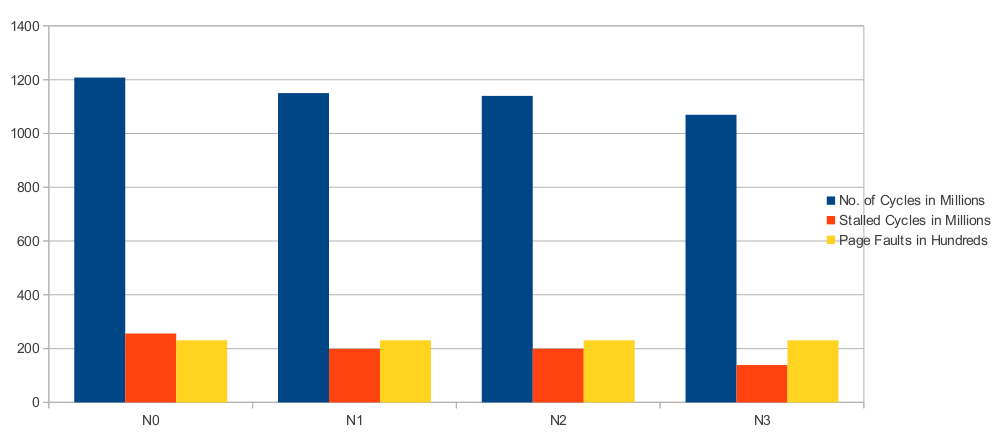
\includegraphics[scale=0.35]{remoteVsLocal.png}
    \caption{Comparision of remote vs local library. Shared library is at N3 }
    \label{fig:remoteVsLocal}
\end{figure}


In the above section we saw the interconnect overhead in terms of slowdown, when we try to fetch data from remote node.
Similar overhead exist in the case when read-only data is being fetched from remote node.
Here our read-only data is the shared library's instructions.
The shared library was placed on Node03 and then we ran the main thread on each of the four nodes.
Main thread called 0.1 million functions from the library in sequential order.
Figure \ref{fig:remoteVsLocal} shows the result.
We measured the total number of CPU cycles consumed, stalled cycles and page faults in each case.
We observed that in the case when our main thread was running locally (i.e. on Node03) minimum number of CPU cycles were consumed, and stalled cycles were also minimum.
We measured page faults to make sure that we are fetching equal number of library pages in all four cases, and number of page faults were equal in all four cases.
The number of cycles consumed were proportional to the interconnect slowdown we saw in above section.
Maximum cycles are consumed for farthest node (accessed via 2 hop) and least for the local node.



\subsection{Small vs Big functions in Library}

\begin{figure}
    \centering
    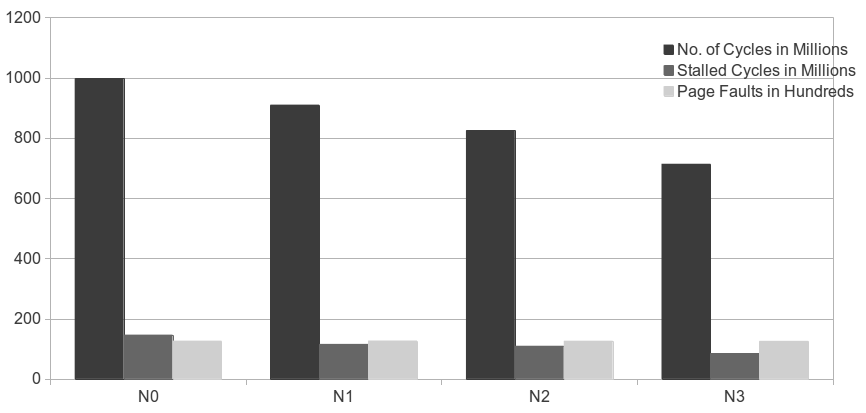
\includegraphics[scale=0.35]{smallFunc.png}
    \caption{Performance with small sized functions. Shared library is at N3 }
    \label{fig:smallFunc}
\end{figure}

The size of each function in above section is about 600 Bytes.
We tried to make smallest possible functions which look like this:

\texttt{ int f0()\{return 0;\} }

with size of 138 Bytes for each function.
With small sized functions we wanted to see if instruction prefetching can help to even out the impact of remote library fetch.
Figure \ref{fig:smallFunc} shows the result.
Experimental settings were similar to section \ref{sec:remoteVsLocal}, shared library was on Node03 and we ran main thread on each of the four nodes.
The results we observed showed similar behavior as in section \ref{sec:remoteVsLocal}.
Number of CPU cycles consumed by remote nodes were more than those consumed by the local nodes.



\subsection{Various probability distributions of function calls}

\begin{figure}
    \centering
    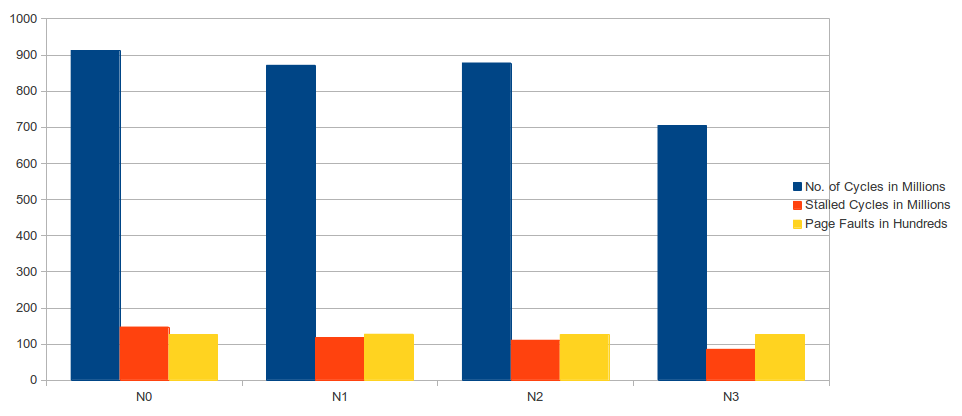
\includegraphics[scale=0.35]{randomDistribution.png}
    \caption{Library functions called in random order by main thread. Shared library is at N3 }
    \label{fig:randomDistribution}
\end{figure}

\begin{figure}
    \centering
    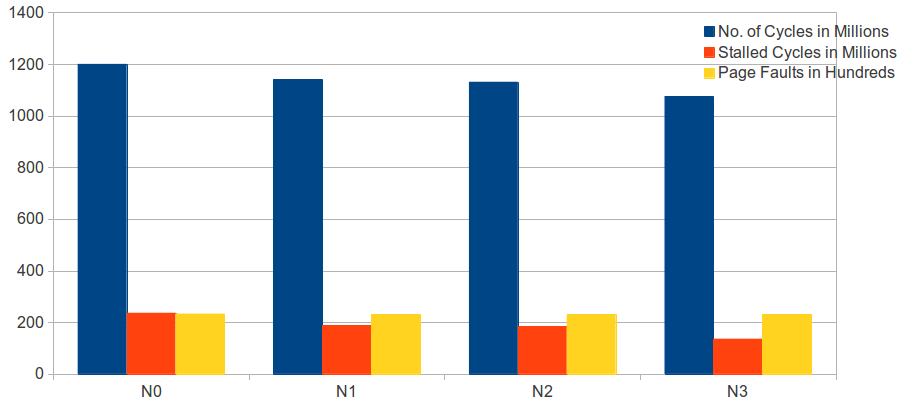
\includegraphics[scale=0.35]{zipfDistribution.png}
    \caption{Library functions called in Zipfian order (with alpha=0.5) by main thread. Shared library is at N3 }
    \label{fig:zipfDistribution}
\end{figure}

Till now we were calling the functions from the shared library in sequential order.
We wanted to vary our function calling pattern to random and zipfian distributions.
In reality it is not necessary that an application is using all the functions of a library and in sequential order.
Instruction caching favours sequential order and to negate the effect of caching we wanted to test random and zipfian distributions.

\textbf{Sequential} - Figure \ref{fig:remoteVsLocal} shows the results for sequential calling pattern

\textbf{Random} - Figure \ref{fig:randomDistribution} shows the results for calling library functions in random order.
The difference in the CPU cycles consumed by N3 (local) and N0,N1,N2 (remote) looks more pronounced.

\textbf{Zipf} - Figure \ref{fig:zipfDistribution} shows the results for calling library functions in zipfian order.
According to zipfian distribution there will be a bunch of functions which will be called more frequently than others.
Therefore instruction caching will favour the performance in this case.
Due to which the difference in the CPU cycles consumed by N3 (local) and N0,N1,N2 (remote) is not great.



